\capa

% \pretextualchapter{}

\folhaderosto
% 
\pretextualchapter{}
	\thispagestyle{plain}
	\noindent \parbox{5.7in}{\centering AUTORIZO A REPRODUÇÃO E DIVULGAÇÃO TOTAL OU PARCIAL DESTE TRABALHO, POR QUALQUER MEIO CONVENCIONAL OU ELETRÔNICO, PARA FINS DE ESTUDO E PESQUISA, DESDE QUE CITADA A FONTE.}

%\pretextualchapter{}



%\afterpage{\blankpage}
%
%\pretextualchapter{DEDICATÓRIA} %Título da página dedicatória
%	\input{dedicatoria} %Para incluir o texto de dedicatória,use o arquivo dedicatória.tex

%\afterpage{\blankpage}


\pretextualchapter{\centerline{AGRADECIMENTOS}} %Título da página de agradecimentos
	
Sinceros agradecimentos ao Prof. Gonzalo Travieso e ao Prof. Luciano da Fontoura
Costa. Tenham certeza que foi com vocês que aprendi o que é fazer
pesquisa. Foram ensinamentos que guardarei para toda a vida. Além da orientação
de excelência, ficará para sempre a amizade.

\vspace{4 mm}

Aos meus queridos pais, Vilson e Salete, sabem que devo tudo o que sou a
vocês. Encontro sempre suas palavras de conforto e sabedoria em cada esquina que
cruzo, em cada caminho que percorro. Amo muito vocês.

\vspace{4 mm}

À minha amada, Gabriela, que esteve ao meu lado em cada momento, bom ou ruim,
por seu amparo, carinho e cumplicidade. Te amo.

\vspace{4 mm}

À Paulo e Lourdes pelas conversas sempre animadas, e à Isabela pelas
risadas sempre prontas às minhas piadas :-D

\vspace{4 mm}

Aos meus irmãos Renato e Ricardo Fabbri, que me acolhem com tanto carinho e com
quem espero viver ainda ótimas passagens. Renato, obrigado por ser um verdadeiro
mentor.

\vspace{4 mm}

Ao bom amigo e conselheiro Pedro Kroeger, continuas sendo a quem sigo os passos.

\vspace{4 mm}

A todos do labMacambira.sf.net, por todas as colaborações e aprendizados, seja
artisticamente, cientificamente, socialmente, em \emph{software},
em \emph{tinta}, em \emph{notas} ou em \emph{espírito}.

\vspace{4 mm}

À Mozilla Foundation e seus colaboradores, em especial ao bom amigo Forrest
Oliphant, que me mentorou enquanto participante do Googler Summer of Code 2012 e
com quem continuo compartilhando ótimas conversas e desenvolvimentos. Thank you Fo!

\vspace{4 mm}

A todos os amigos que fiz no IFSC/USP, em especial Carlos Doro Neto (valeu
pelo \textit{Doro's method}!), David Sbrissa (\textit{bit******!}),
prof. Osvaldo ``Chu'', prof. Rodrigo Guido, profa. Yvonne Mascarenhas, Débora
Correa, Mauro Miazaki, Diego, César, Thomás, Filipi. Aos parceiros
do \textit{hacklab do velho}, tenho grande carinho por todos vocês.

\vspace{4 mm}

Não sei se conseguirei lembrar de todos, mas meu especial agradecimento e grande
carinho a Daniel Penalva, Caleb Luporini, Guilherme Lunhani, Geraldo Magela
Rocha, Glerm Soares, Chico e Fábio Simões, Daniel Marostegan, prof. Rogério
``Zeco'' Silva, Gilson Beck, Marcos Mendonça, Danilo Shiga, Edson Corrêa,
Vanessa Ferreira, prof. Luis Castelões, Luis Fernando Muniz Cirne, Marília
Pisani, prof. Massimo Canevacci. À Teia Casa de Criação e Pontão Nós Digitais,
ao MuSA, aos amigos da Udesc, à galera do AVAV, do Crânio Sonante, a todos que
tive contato real e virtualmente, nas listas de email, AA, IRC e outras redes e
canais.

\vspace{4 mm}

Agradeço às comunidades de cultura e software livre e aberto por todos os
conhecimentos e tecnologias repassados e que compõem esta contribuição.

\vspace{4 mm}

\begin{center}
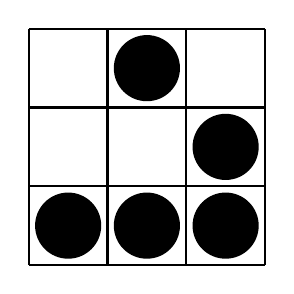
\begin{tikzpicture}[thick]
\draw (0,0) grid (3,3);
\foreach \c in {(0,0), (1,0), (2,0), (2,1), (1,2)}
    \fill \c + (0.5,0.5) circle (0.42);
\end{tikzpicture}
\end{center}
 %Para incluir o texto de agradecimentos,use o arquivo agradecimentos.tex


\pretextualchapter{}
	\begin{epigrafetop}
		{A arte é feita para perturbar. A ciência tranquiliza. Na arte só uma coisa importa: aquilo que não se pode explicar.}
        {Goerges Braque}
	\end{epigrafetop}

	\begin{epigrafemid}
		{A ciência é tudo aquilo que conseguimos explicar a um computador. Todo o resto é arte.}
		{Donald Knuth}
	\end{epigrafemid}
	\vspace{-1cm}

	\begin{epigrafebot}
                {Todos querem entender de arte. Por que não tentam entender o
                canto de um pássaro?}
                {Pablo Picasso}
	\end{epigrafebot}



\afterpage{\blankpage}

\resumoeabstract %Para incluir o texto do resumo e abstract,use o arquivo resumoeabstract.tex

\afterpage{\blankpage}


\listadefiguras %Comando que gera a lista de figuras (AUTOMÁTICO)

%\afterpage{\blankpage}
\listadetabelas %Comando que gera a lista de tabelas (AUTOMÁTICO)

\afterpage{\blankpage}

\renewcommand{\contentsname}{\hspace*{\fill}SUMÁRIO\hspace*{\fill}}
\sumario

